\scanpage{3}
\margin{\figure{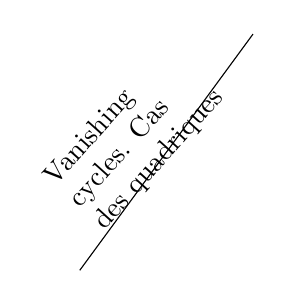
\begin{tikzpicture}[baseline]
\draw (0,0)--(2.2,3);
\node[rotate=48,anchor=west,align=left] at(-.15,.75)
{\uline{Vanishing}\\cycles. Cas\\des quadriques};
\end{tikzpicture}}}
\diagram{\begin{tikzcd}X\arrow[d,"f"]\\S\end{tikzcd}}
$f$ morphisme projectif plat

$S$ spectre d'un anneau de val discrète strictement local

$X_0$ fibre spéciale quadrique à point singulier

$\bar X_1$ fibre géom générique, quadrique non singulière

dimension commune des fibres $n-1$

\unsure{\big[}
\deleted{\unsure{On veut étudier}}
$X\deleted{\unsure{n}}\subset\mathbf P^n_S$ défini par une équation quadratique \ldots

\[
H^i(X_0)\mathbin{-}H^i(\bar X_1)\qquad ?
\]
On a la suite exacte générale
\[
\cdots\mathbin{-}H^i(X_0)\mathbin{-}H^i(\bar X_1)
\mathbin{-}\Phi^{i+1}\mathbin{-}H^{i+1}(X_0)
\mathbin{-}H^{i+1}(\bar X_1)\mathbin{-}\cdots
\]
On sait que la cohomologie de \deleted{$H^*(X_0)$ et}
\deleted{1°) \uline{$n$ pair}, \unsure{donc $n-1$ impair}}
$X_0$ et $\bar X_1$ est nulle en dim impaires. Donc
on trouve
\[
0\longrightarrow\Phi^{2\nu}\longrightarrow H^{2\nu}(X_0)
\mathbin{-}H^{2\nu}(\bar X_1)\longrightarrow\Phi^{2\nu+1}\mathbin{-}0
\]
i.e. les $\Phi^i$ apparaissent exactement comme les
noyaux et conoyaux du \uline{hom. de spécialisation}.

Notons aussi que sur $X$ donc $X_0$, on a une
classe $\xi\in H^2(X,\unsure{\mu}(1))$, provenant de la section
à l'infini, et dont la restriction à chaque fibre
est connue \ldots
\margin{2}
